\documentclass[a4paper]{article}

\usepackage[fontset=fandol]{ctex}
\usepackage{amsmath, amssymb}
\usepackage{graphicx}
\usepackage[margin=2.3cm]{geometry}
\usepackage[most]{tcolorbox}
\usepackage{etoolbox}
\usepackage{listings}
\usepackage{hyperref}
\usepackage{xurl}
\usepackage{booktabs}
\usepackage{longtable}
\usepackage{tabularx}
\usepackage{array}
\usepackage{subcaption}
\usepackage{float}
\usepackage{enumitem}
\usepackage{tikz}
\usetikzlibrary{arrows.meta, positioning, shapes.geometric, fit}
\IfFileExists{pgfplots.sty}{
    \usepackage{pgfplots}
    \pgfplotsset{compat=1.18}
}{}

\hypersetup{
    colorlinks=true,
    linkcolor=blue!50!black,
    urlcolor=blue!60!black,
    citecolor=blue!50!black
}

\newtcolorbox{findingbox}[1]{
    enhanced,
    colback=green!5!white,
    colframe=green!45!black,
    colbacktitle=green!45!black,
    coltitle=white,
    fonttitle=\bfseries,
    title=#1,
    sharp corners
}

\newtcolorbox{evidencebox}[1]{
    enhanced,
    colback=blue!4!white,
    colframe=blue!65!black,
    colbacktitle=blue!65!black,
    coltitle=white,
    fonttitle=\bfseries,
    title=#1,
    sharp corners
}

\newtcolorbox{riskbox}[1]{
    enhanced,
    colback=red!4!white,
    colframe=red!70!black,
    colbacktitle=red!70!black,
    coltitle=white,
    fonttitle=\bfseries,
    title=#1,
    sharp corners
}

\newtcolorbox{methodbox}[1]{
    enhanced,
    colback=yellow!9!white,
    colframe=yellow!60!black,
    colbacktitle=yellow!60!black,
    coltitle=black,
    fonttitle=\bfseries,
    title=#1,
    sharp corners
}

\lstset{
    language=Python,
    basicstyle=\ttfamily\small,
    keywordstyle=\color{blue},
    stringstyle=\color{red!60!black},
    commentstyle=\color{green!50!black},
    breaklines=true,
    frame=single,
    numbers=left,
    numberstyle=\tiny\color{gray},
    captionpos=b,
    extendedchars=false
}

\newcolumntype{Y}{>{\raggedright\arraybackslash}X}
\setlist[itemize]{leftmargin=1.8em}

\newcommand{\reporttitle}{视频结构切分、镜头边界与场景分段深度研究}
\newcommand{\reportsubtitle}{从 TransNetV2 / PySceneDetect 到 scene-level VLM：benchmark、论文谱系、工程项目与 video-note 落地路线}
\newcommand{\reportauthors}{Codex}
\newcommand{\reportdate}{2026-03-26}
\newcommand{\researchquestion}{如果目标是为后续视频笔记、关键帧提取、章节组织和 PDF 构建服务，应该如何理解并组合 shot boundary detection、scene segmentation、slide/keyframe extraction 这几个方向？}
\newcommand{\reportscope}{研究范围覆盖截至 2026-03-26 的公开 benchmark、核心论文、官方项目文档和本地 video-note case。重点不在“纯学术排名”，而在这些技术对真实视频处理链路的价值、边界和可复现接入方式。}
\newcommand{\reportaudience}{需要设计或升级视频结构化处理方案的工程负责人、agent skill 维护者，以及后续要把视频转成讲义 / 笔记 / 章节化摘要的人}
\newcommand{\sourcewindow}{外部资料访问日期为 2026-03-26；本地案例与仓库状态截至 2026-03-26}
\newcommand{\reportcoverpath}{figures/cover-collage.jpg}

\begin{document}

\begin{titlepage}
\centering
{\Large 深度研究报告\par}
\vspace{1.0cm}
{\huge\bfseries \reporttitle\par}
\vspace{0.5cm}
{\Large \reportsubtitle\par}
\vspace{0.9cm}
{\large \reportauthors\par}
\vspace{0.2cm}
{\large \reportdate\par}
\vspace{1.0cm}
\includegraphics[width=0.9\textwidth,height=0.42\textheight,keepaspectratio]{\reportcoverpath}\par
\vfill
\begin{tcolorbox}[width=0.94\textwidth, colback=black!2!white, colframe=black!60, sharp corners]
\textbf{核心问题}：\researchquestion\par
\textbf{研究范围}：\reportscope\par
\textbf{目标读者}：\reportaudience\par
\textbf{证据窗口}：\sourcewindow\par
\end{tcolorbox}
\end{titlepage}

\tableofcontents
\newpage

\section{执行摘要}

\begin{findingbox}{最重要的结论}
如果你的目标是“让视频处理链路更稳定地产出讲义、关键图和章节结构”，那么不应把 \textbf{shot boundary detection} 直接等同于“解决方案本身”。它更适合充当一个中间层能力：发现视觉切换点、帮助路由 case、缩小候选时间窗；真正决定最终质量的，仍然是 \textbf{字幕/转写、视觉模式识别、裁剪/OCR/layout、以及文档叙事层} 的组合。
\end{findingbox}

\begin{itemize}
\item 公开社区里，\textbf{低层 shot boundary detection 已经比较成熟且增量放缓}。经典 benchmark 的主线大致是：DeepSBD / DSM $\rightarrow$ TransNet $\rightarrow$ TransNetV2 $\rightarrow$ AutoShot。到 2023 年，AutoShot 仍是公开可复现、且在短视频场景里最有代表性的 SBD 更新点。
\item 近两年的研究重心明显往上移动，更多工作在做 \textbf{scene segmentation、generic event boundaries、甚至 vision-language based scene understanding}。这说明社区正在从“找镜头断点”转向“理解叙事单元和语义边界”。
\item 截至 2026-03-26，\textbf{2025 年之后最值得跟踪的公开模型并不在纯 shot-level}。我这次追到的主线分别是：AAAI 2025 的 MASRC 把 MovieNet / MovieScenes 这条 scene detection 线继续往前推；ICCV 2025 的 DiffGEBD、ESTimator 与 arXiv 2025 的 Structured Context Learning 把边界研究推向 GEBD 和在线边界；而 Scene-VLM 则把 scene segmentation 推向 7B 级多模态 VLM。
\item 对 video-note 场景而言，\textbf{PySceneDetect 和 FFmpeg 的 ROI 高于一开始就接入学习型模型}。它们足以作为 `cheap probe` 来判断一个视频是否需要更密集的候选帧搜索、是否存在明显的视觉段落，以及该走哪条后续分支。
\item \textbf{TransNetV2 值得调研但不该作为第一优先级接入}。它在 benchmark 上很强，但官方 inference 仍旧绑定老 TensorFlow 2.1 / git-lfs 权重；而且对 `static-outline`、`board-heavy` 这类知识讲解视频，镜头边界往往不等于“高价值讲义图片”。
\item 最适合你当前链路的方案不是“只换模型”，而是先补上一个\textbf{稳定的结构化中间层}：`decode-normalize -> cheap boundary probe -> mode routing -> candidate windows -> crop/OCR/layout -> render manifest`。
\end{itemize}

\begin{riskbox}{需要特别避免的误区}
如果只盯着 benchmark F1 排名，很容易忽略两个更现实的问题：第一，真实 B 站 / YouTube 视频的编码、分辨率、画中画布局、字幕质量和平台下载限制会直接决定工具能否跑通；第二，即便镜头边界检测非常准，也不一定能给讲义带来更好的图示，因为很多知识视频的关键价值来自同一页 slide 的渐进展开、白板累积、或口播论证结构，而不是镜头切换本身。
\end{riskbox}

\section{研究范围、方法与术语边界}

\subsection{为什么这个方向容易被混淆}

用户给出的两个入口分别是 \href{https://github.com/soCzech/TransNetV2/blob/master/README.md}{TransNetV2} 和 \href{https://www.scenedetect.com/}{PySceneDetect}。它们都和“视频切分”有关，但并不等价：

\begin{itemize}
\item 前者更偏 \textbf{shot boundary detection}，即找到镜头切换或转场；
\item 后者是更工程化的 \textbf{scene detection toolkit}，覆盖内容差异、淡入淡出、hash/histogram 等若干启发式检测器；
\item 而你本地 video-note 背景报告已经说明，真实任务还涉及 \textbf{slide/keyframe extraction、candidate window narrowing、crop/OCR/layout、PDF 叙事组织}。
\end{itemize}

因此本报告不把这些问题混成一个“视频切分”筐，而是把领域拆成四层。

\begin{table}[H]
\centering
\small
\begin{tabularx}{\textwidth}{p{2.8cm}p{3.0cm}p{2.8cm}Y}
\toprule
层级 & 典型输出 & 代表 benchmark / 项目 & 对 video-note 的意义 \\
\midrule
Shot boundary detection & cut / gradual transition 时间点 & BBC, RAI, ClipShots, SHOT; TransNetV2, AutoShot & 适合找视觉断点、缩小候选窗口，但不直接等于“讲义图” \\
Scene segmentation & 语义场景边界、章节段落 & MovieScenes / MovieNet-SSeg, OVSD, BBC scene benchmark & 更接近你想要的“章节组织”与叙事结构 \\
GEBD / generic event boundaries & 人感知的重要事件边界 & Kinetics-GEBD 等 & 与 shot 不同，更偏事件理解，适合交互或 highlight 场景 \\
Slide / keyframe extraction & 代表帧、去重 slide、裁剪图 & Lecture2Notes 风格流程、FFmpeg / PySceneDetect / OCR 组合 & 对生成 PDF、图示与页面素材最直接 \\
\bottomrule
\end{tabularx}
\caption{这几个相关方向共享“边界”概念，但工程目标并不相同。对于讲义生成，真正要组合的是多层技术而不是押注单一 SBD 模型。}
\end{table}

\subsection{证据来源与本地实验}

\begin{methodbox}{证据组成}
\begin{itemize}
\item 本地背景材料：已有 \texttt{video-note-visualize-deepresearch} 报告、\texttt{video-note-pipeline} README、多个 retrospective case。
\item 官方项目与文档：TransNetV2、PySceneDetect、FFmpeg、AutoShot、ClipShots。
\item 论文：TransNetV2、AutoShot、ClipShots、MovieNet / MovieScenes、Neighbor Relations Matter、Scene-VLM。
\item 本地实验：在 \texttt{BV1oTwkzvEFu} 样例视频上，分别运行 FFmpeg scene score 扫描与 PySceneDetect content/adaptive detector，对比实际边界数量和接入摩擦。
\end{itemize}
\end{methodbox}

\subsection{benchmark 常用指标}

Shot boundary 与 scene segmentation 常见指标并不完全一致，但最常用的两个是 F1 和 AP。

$$
F1 = \frac{2PR}{P + R}
$$

\begin{itemize}
\item $P$：precision，检测出的边界里有多少是真边界
\item $R$：recall，真实边界里有多少被检测到
\item $F1$：同时平衡精确率和召回率的调和平均
\end{itemize}

在 movie scene segmentation 里，还常见 AP、mIoU、Recall@3s 等指标。它们比单纯 F1 更关注排序质量、边界容差和长视频语义段落的一致性。

\begin{evidencebox}{为什么不能只看一个数字}
BBC / RAI 这类数据集相对静态，很多方法都接近饱和；ClipShots 和 SHOT 则更接近互联网视频与短视频场景；MovieNet-SSeg 又从“镜头断点”升级到了“叙事场景边界”。如果不先区分 benchmark 性质，再比较数字，很容易得到错误路线。
\end{evidencebox}

\section{Benchmark 图谱：这个领域到底在测什么}

\subsection{Shot-level benchmark：从静态电视节目到互联网短视频}

\begin{table}[H]
\centering
\small
\begin{tabularx}{\textwidth}{p{2.2cm}p{2.7cm}p{3.0cm}p{2.7cm}Y}
\toprule
数据集 & 内容类型 & 规模 / 标注 & 常用指标 & 适合作为什么能力测试 \\
\midrule
BBC Planet Earth & 纪录片 / 教育电视 & 11 集，每集约 50 分钟，约 4900 shots、670 scenes & F1 & 低噪声、相对静态的镜头边界检测 \\
RAI & 广播 / talk show & 10 个广播视频，单视频约半小时；ClipShots 论文给出 722 cut + 263 gradual & F1 & 老牌 benchmark，规模较小，容易接近饱和 \\
ClipShots & YouTube / Weibo 多类型互联网视频 & 4039 视频，128636 cut + 38120 gradual；测试集 500 视频，5876 cut + 2422 gradual & F1 / cut-gradual 分项 & 更接近开放互联网视频，难度显著高于 BBC / RAI \\
SHOT & 短视频平台内容 & 853 条短视频，11606 shot annotations；200 条测试视频含 2716 高质量边界标注 & F1、固定 recall 下 precision & 对短视频、高频转场、复杂编辑更敏感 \\
\bottomrule
\end{tabularx}
\caption{Shot-level benchmark 主要回答“哪里发生了视觉转场”。数据来源：ClipShots 论文与 README、AutoShot 论文与 README。}
\end{table}

\begin{riskbox}{benchmark 饱和的工程含义}
如果一个方法只在 BBC / RAI 上看起来很强，并不意味着它对你的视频就更有用。对 video-note 链路更有参考价值的，是 ClipShots / SHOT 这类互联网和短视频分布，以及你自己的历史 case。
\end{riskbox}

\subsection{公开可复现的 shot-level 对比结果}

\begin{figure}[H]
\centering
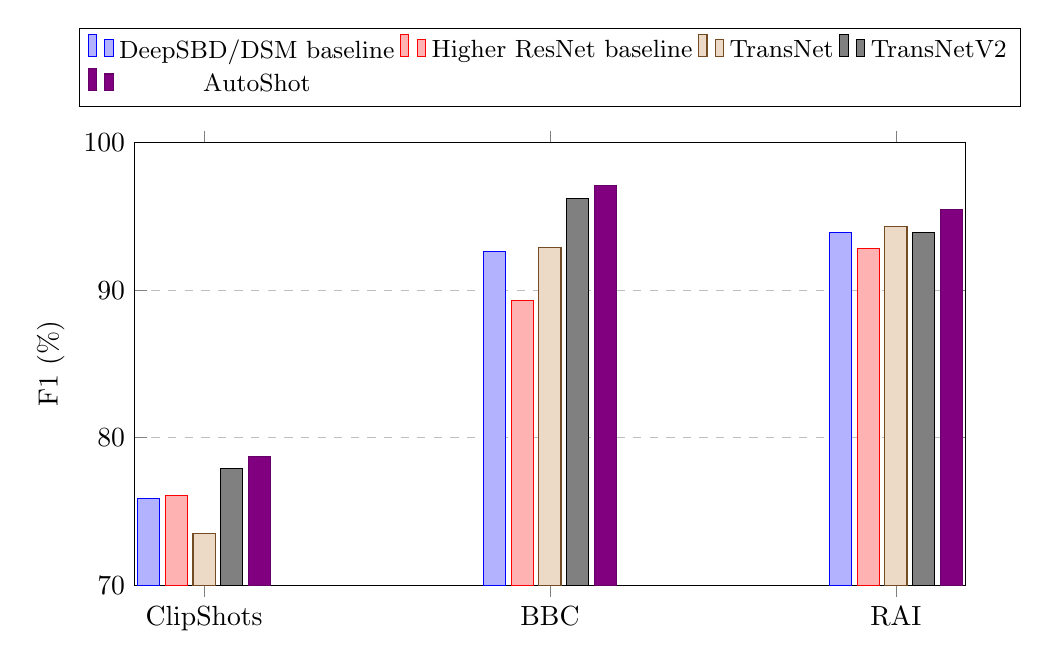
\begin{tikzpicture}
\begin{axis}[
    ybar,
    bar width=8pt,
    width=\textwidth,
    height=7.2cm,
    ymin=70,
    ymax=100,
    symbolic x coords={ClipShots,BBC,RAI},
    xtick=data,
    ylabel={F1 (\%)},
    legend style={at={(0.5,1.08)}, anchor=south, legend columns=4, font=\small},
    ymajorgrids=true,
    grid style=dashed,
]
\addplot coordinates {(ClipShots,75.9) (BBC,92.6) (RAI,93.9)};
\addplot coordinates {(ClipShots,76.1) (BBC,89.3) (RAI,92.8)};
\addplot coordinates {(ClipShots,73.5) (BBC,92.9) (RAI,94.3)};
\addplot coordinates {(ClipShots,77.9) (BBC,96.2) (RAI,93.9)};
\addplot coordinates {(ClipShots,78.7) (BBC,97.1) (RAI,95.5)};
\legend{DeepSBD/DSM baseline,Higher ResNet baseline,TransNet,TransNetV2,AutoShot}
\end{axis}
\end{tikzpicture}
\caption{ClipShots / BBC / RAI 上公开常见模型的 F1 对比。来源：TransNetV2 官方 README 与 AutoShot 论文表 2。AutoShot 的数值来自其论文中对 TransNetV2 的 PyTorch 复现结果。}
\end{figure}

\begin{table}[H]
\centering
\small
\begin{tabular}{lcc}
\toprule
模型 & SHOT F1 & 备注 \\
\midrule
TransNetV2 & 0.799 & AutoShot 论文中的对照基线 \\
AutoShot@F1 & 0.841 & 在 SHOT 上比 TransNetV2 高 4.2 个百分点 \\
AutoShot@Precision & 0.826 & 固定 recall 约束下优化 precision 的版本 \\
\bottomrule
\end{tabular}
\caption{SHOT benchmark 上最关键的比较。来源：AutoShot 论文表 2 左。}
\end{table}

\subsection{Scene-level benchmark：研究重心已经往语义边界上移}

从 2020 年之后，很多论文不再只满足于检测 cut / dissolve，而开始把问题提升到 \textbf{scene segmentation}：也就是在一串 shots 里找出真正的叙事场景边界。

\begin{table}[H]
\centering
\small
\begin{tabularx}{\textwidth}{p{2.7cm}p{2.7cm}p{3.0cm}p{2.7cm}Y}
\toprule
数据集 / benchmark & 内容类型 & 规模 & 常用指标 & 与你任务的关系 \\
\midrule
MovieScenes / MovieNet-SSeg & 电影长视频 & 150 部电影，约 270K shots & AP、mIoU、F1、Recall@3s & 更接近“章节 / 段落结构”，适合长视频叙事组织 \\
BBC scene benchmark & 纪录片场景 & BBC Planet Earth 上的 scene annotation & AP 等 & 适合较稳定长视频的 scene-level 比较 \\
OVSD & 短片 / 开放视频场景分段 & 21 部短片 & AP 等 & 更靠近开放视频而非单纯电影 \\
\bottomrule
\end{tabularx}
\caption{Scene-level benchmark 不再只关心镜头切换，而是关心一段叙事何时结束、何时进入下一段。}
\end{table}

\begin{findingbox}{研究趋势判断}
结合 MovieNet / MovieScenes、CVPR 2024 的 \textit{Neighbor Relations Matter in Video Scene Detection}，以及 2026 年已接受的 \textit{Scene-VLM}，可以看出研究主线已经从“单帧或短窗是否为转场”上移到“多 shot 之间的关系建模、跨模态上下文、甚至边界原因解释”。
\end{findingbox}

\section{论文与模型演进}

\subsection{第一阶段：启发式与轻量工程工具仍然很有生命力}

\subsubsection{FFmpeg：最低成本、最高工程确定性的基线}

\href{https://ffmpeg.org/ffmpeg-filters.html}{FFmpeg 官方文档}明确支持基于 \texttt{scene} 分数的筛选，例如 \texttt{select='gt(scene,0.4)'}。这类方法的优点是：

\begin{itemize}
\item 没有重模型依赖，几乎任何环境都能跑；
\item 可以与 \texttt{thumbnail}、\texttt{fps}、\texttt{cropdetect}、\texttt{tile} 直接组合；
\item 非常适合作为 preflight 或 cheap probe。
\end{itemize}

缺点也很明显：阈值高度敏感、对渐进式 reveal 和低变化白板不稳、完全没有语义理解。

\subsubsection{PySceneDetect：最适合落到你现有 pipeline 的第一层增强}

\href{https://www.scenedetect.com/docs/latest/cli.html}{PySceneDetect 官方 CLI 文档}当前至少提供五类检测器：

\begin{itemize}
\item \texttt{detect-content}：基于相邻帧内容差异，默认切 hard cuts；
\item \texttt{detect-adaptive}：先做 content score，再滚动平均，减小相机运动导致的误报；
\item \texttt{detect-threshold}：面向淡入淡出；
\item \texttt{detect-hash}：感知 hash；
\item \texttt{detect-hist}：基于直方图差异。
\end{itemize}

对你来说，它的价值不是“替代全部视频分析”，而是：

\begin{itemize}
\item 在 transcript window 太粗的时候，把视觉窗口再切细一层；
\item 在 mixed slides / mixed speaker 视频里找到真正发生视觉切换的局部；
\item 生成可以被后续 crop / OCR / layout 模块消费的候选时间窗。
\end{itemize}

\subsection{第二阶段：深度学习把 SBD 推到了更强、更快的阶段}

\subsubsection{DeepSBD / DSM / ClipShots：把互联网视频纳入 benchmark}

2017 年的 \textit{Large-scale, Fast and Accurate Shot Boundary Detection through Spatio-temporal Convolutional Neural Networks}（通常被称为 DeepSBD）把问题明确成 sharp / gradual / no-transition 分类。2018 年的 ClipShots / DSM 则进一步把 benchmark 从传统电视节目推向 YouTube / Weibo 视频，并采用 cascade 设计：先做轻量过滤，再分别做 cut detector 和 gradual detector。

这一步的重要意义不是某一个网络结构，而是 \textbf{benchmark 分布的改变}：从静态纪录片转向带手抖、遮挡、家庭拍摄、剪辑效果的开放互联网视频。

\subsubsection{TransNet 与 TransNetV2：今天仍然最值得参考的公开视频 SBD 基线}

\href{https://arxiv.org/abs/2008.04838}{TransNetV2 论文}和官方仓库给出了几个很关键的工程细节：

\begin{itemize}
\item 输入是低分辨率的时序窗口，训练和评估使用 $N=100$ 帧输入；
\item 只取中间 50 帧做预测，以避免窗口边缘的上下文不足；
\item 结构核心是带 dilation 的 DDCNN V2 cell，使用 3D 卷积建模时序；
\item 使用两个 head：single-frame head 和 all-frame head，实际评估主要依赖 single-frame head；
\item 训练时混合真实 transitions 与大量人工合成的 hard cut / dissolve。
\end{itemize}

\begin{evidencebox}{为什么 TransNetV2 到今天仍重要}
它不是最新年份的论文，但它同时满足三点：benchmark 够强、仓库够完整、工程语义够清晰。对于想从“无结构的 ffmpeg heuristics”迈向“有学习能力的 SBD”的团队，它仍然是很好的认知基线。
\end{evidencebox}

\subsubsection{AutoShot：短视频时代最有代表性的 shot-level 更新}

\href{https://arxiv.org/abs/2304.06116}{AutoShot} 做了两件非常重要的事：

\begin{itemize}
\item 发布了面向短视频平台的 SHOT 数据集：853 条完整短视频，11606 个 shot 标注，200 条测试视频包含 2716 个高质量边界标注；
\item 通过 neural architecture search，在 3D ConvNet 与 Transformer 构成的搜索空间上寻找更适合短视频 SBD 的结构。
\end{itemize}

其论文表明：

\begin{itemize}
\item 在 SHOT 上，AutoShot 的 F1 比 TransNetV2 高 4.2 个百分点；
\item 在 ClipShots / BBC / RAI 上，也分别比之前的最好结果再高 1.1 / 0.9 / 1.2 个百分点。
\end{itemize}

这说明短视频不是“把老 benchmark 再做一遍”就能解决的；它们需要显式面向高频转场、复杂编辑风格和更短 shot length 的模型设计。

\subsection{第三阶段：研究前沿上移到 scene segmentation 与 VLM}

\subsubsection{MovieNet / MovieScenes：从镜头断点到叙事场景}

\href{https://arxiv.org/abs/2004.02678}{MovieNet / MovieScenes 论文}把 scene segmentation 放到 150 部电影、约 270K shots 的规模上来做。它的关键判断是：\textbf{shot boundary 是视觉切换，scene boundary 是叙事切换，两者并不等价。}

这和你的场景非常相关。因为 video-note 真正想要的通常不是“第几帧切了镜头”，而是：

\begin{itemize}
\item 这一段开始讲一个新话题了吗；
\item 这一页 slide 的展开是否进入了一个新的解释单元；
\item 这一部分是否值得新开一个章节或小节。
\end{itemize}

\subsubsection{Neighbor Relations Matter (CVPR 2024)：关系建模比纯邻近分数更重要}

\href{https://openaccess.thecvf.com/content/CVPR2024/html/Tan_Neighbor_Relations_Matter_in_Video_Scene_Detection_CVPR_2024_paper.html}{Neighbor Relations Matter in Video Scene Detection} 在 MovieNet 上报告了较强结果。其核心思想不是再堆一个更大的 encoder，而是显式建模不同 shot 之间的近邻关系和时间图结构。

论文结果显示，在 MovieNet 的 fully supervised setting 下，作者方法相对于 LGSS、Temporal Perceiver、MHRT 等更早方法有明显提升。这说明 \textbf{scene detection 的瓶颈已经不是“能不能看见切换”，而是“能否理解跨 shot 的关系”}。

\subsubsection{Scene-VLM (CVPR 2026 accepted)：前沿正在转向多模态与可解释}

根据 \href{https://arxiv.org/abs/2512.21778}{Scene-VLM 的 arXiv 摘要}，该工作提出了面向视频 scene segmentation 的 VLM 框架，同时利用帧、转写文本与可选 metadata，并且能输出边界判断的自然语言 rationale。摘要直接报告，在 MovieNet 上相对前一代方法有约 \textbf{+6 AP 和 +13.7 F1} 的提升。

\begin{findingbox}{这对你意味着什么}
如果你未来想做的不是“多找几个 cut”，而是“让 agent 更像人在整理一场讲座或一次视频材料”，那么真正有潜力的长期路线不是更极致的 shot detector，而是 scene-level、多模态、可解释的边界理解。
\end{findingbox}

\subsection{第四阶段：2025+ 模型与 baseline 继承链}

\begin{findingbox}{2025+ 最重要的判断}
如果只看“最近有没有新模型”，会误以为 shot boundary detection 仍是主战场。实际上截至 2026-03-26，公开论文里最明显的增量来自 \textbf{scene segmentation} 与 \textbf{GEBD}。从 arXiv 最近检索结果看，纯 \textbf{shot boundary detection} 的公开主流方法仍基本停留在 2023 年的 AutoShot，而 2025 年之后的新强模型主要在更高层的语义边界任务上竞争。
\end{findingbox}

\begin{table}[H]
\centering
\scriptsize
\begin{tabularx}{\textwidth}{p{2.4cm}p{2.0cm}p{3.5cm}p{3.3cm}Y}
\toprule
模型 / 年份 & 任务层级 & 主要 baseline / 对比对象 & 代表性结果 & 强度判断与工程含义 \\
\midrule
MASRC (AAAI 2025) & Video scene detection & ShotCoL、SCRL、BaSSL、TranS4mer、VSMBD、NeighborNet、Temporal Perceiver、MHRT、CANet & MovieNet self-supervised transfer：AP 73.2 / mIoU 70.7 / F1 67.3；BBC 零样本 AP 53.2，OVSD AP 48.3 & 这是我本轮检索到最像“现代 scene-level 实用基线”的 2025 模型：参数量只有 21.4M（entity+place），并且官方 repo 已公开；但依赖 MovieNet shot features，接入前要先有 shot/feature 中间层。 \\
Scene-VLM (arXiv 2025, CVPR 2026 accepted) & Multimodal scene segmentation & Chapter-LLaMA、LGSS、ShotCoL、BaSSL、MEGA、TranS4mer & MovieNet-318：F1 62.1 / AP 66.8；相对 MEGA +6.8 F1 / +8.2 AP，相对 TranS4mer +13.7 F1 / +6.0 AP；BBC zero-shot AP 45.8 & 从语义能力和解释性看，这是 inspected sources 里最强的 frontier；但文中 7B 版本需要 16--18 GB 峰值显存，10 个决策约 1.84--2.34 秒，明显比编码器型 scene model 更重。 \\
Structured Context Learning (2025) & GEBD + adjacent shot benchmark & PC、PC+OF、UBoCo、Com-Net、DDM-Net、TP-Net、MA-Net、BasicGEBD；以及 TransNet / TransNetV2 & Kinetics-GEBD Avg 0.883；TAPOS Avg 0.745；ClipShots / BBC / RAI F1 = 79.5 / 98.4 / 96.2 & 它说明“边界研究”并没有停，只是研究对象已从 SBD 扩展到 generic event boundaries。值得注意的是，它仍保留了对 TransNetV2 的 shot benchmark 对比，因此很适合拿来说明两个赛道如何衔接。 \\
ESTimator (ICCV 2025) & Online GEBD & TeSTra-BC、Sim-On-BC、OadTR-BC、MiniROAD-BC；并与 PC / SceneDetect 等 offline 方法对照 & 在线 Kinetics-GEBD Avg 0.748，对比 MiniROAD-BC 的 0.681；在线 TAPOS Avg 0.547，对比 MiniROAD-BC 的 0.528 & 如果你以后要做流式章节提示、实时剪辑提醒或边看边记，这条线比离线 scene detector 更 relevant；但对当前离线 video-note pipeline 不是第一优先级。 \\
DiffGEBD (ICCV 2025) & Diversity-aware GEBD & BasicGEBD、EfficientGEBD、SC-Transformer、DDM-Net、Temporal Perceiver & Conventional GEBD：Kinetics F1@0.05 = 78.4，TAPOS = 65.8；Diversity-aware：F1sym 74.0，Diversity 20.4 & 这是 2025 GEBD 里最有新意的一条线，因为它不只追单一 F1，还显式建模“多个合理边界答案”。官方 repo 已公开，但范式更适合研究人感知边界，而不是直接拿来替代讲义场景的候选窗模块。 \\
\bottomrule
\end{tabularx}
\caption{2025 年及以后的主要公开模型，需要按任务层级拆开看，而不是混成一个“视频切分 SOTA”。}
\end{table}

\subsubsection{这些新论文到底拿谁做 baseline}

\begin{itemize}
\item \textbf{MASRC (AAAI 2025)} 已经不再拿 TransNetV2 或 AutoShot 当主要竞争对手，而是沿着 MovieNet / MovieScenes 这条 \textbf{scene detection} 线，和 ShotCoL、SCRL、BaSSL、TranS4mer、VSMBD、NeighborNet 这些方法比较。更重要的是，它在同一篇论文里同时给出 self-supervision、fully supervision、self-supervised transfer 三个 setting 的表格，不是只挑一个 setting 取巧。仓库内部还保留了 \texttt{LGSS.py} 与 \texttt{SCRL} 等模块命名，说明它工程上直接站在既有 scene segmentation 谱系之上，而不是另起一套完全无关的代码。
\item \textbf{Scene-VLM} 的 baseline 链进一步上移。它对比的是 LGSS、ShotCoL、BaSSL、MEGA、TranS4mer 和 Chapter-LLaMA，而不是传统 shot detector。这是最强的任务迁移信号之一：前沿问题已经从“这个局部是不是 cut”转成“这串 shots 是否构成新 scene、能否用文本和人物信息解释边界”。
\item \textbf{Structured Context Learning} 很有代表性，因为它同时跨了两条线：在 Kinetics-GEBD / TAPOS 上对比 PC、DDM-Net、TP-Net、BasicGEBD 这一系 GEBD 方法；在 ClipShots / BBC / RAI 上又保留了对 TransNet、TransNetV2 的比较。因此它很适合解释一个现实情况：最近两年的边界研究并不是抛弃 SBD，而是把 SBD 变成了相邻 benchmark 或下游子问题。
\item \textbf{ESTimator} 的 baseline 选择完全变了：它主要拿 TeSTra、Sim-On、OadTR、MiniROAD 这些 \textbf{在线视频理解 / 在线动作定位} 方法来改造比较。这意味着一旦任务被定义成 streaming 场景，原有的离线 scene detector 谱系就不再是最直接的对手。
\item \textbf{DiffGEBD} 的谱系也很清楚。官方 repo 明确写到构建在 \texttt{EfficientGEBD} 代码库之上；论文主表则继续和 BasicGEBD、SC-Transformer、DDM-Net 比。这条线的创新点不是“换了一个更大的 backbone”，而是把边界预测改造成生成式、多解式问题，并引入 symmetric F1 / diversity 这样的新评价方式。
\end{itemize}

\begin{evidencebox}{对“最近模型强不强”的正确读法}
MASRC、Scene-VLM、Structured Context Learning、ESTimator、DiffGEBD 都算近两年的强工作，但它们强在\textbf{不同层级的问题}上：MASRC / Scene-VLM 强在 scene segmentation；Structured Context Learning / DiffGEBD 强在 GEBD；ESTimator 强在在线 GEBD。只有把 benchmark、输入假设、输出定义和推理成本一起看，“强度”这个词才有工程意义。
\end{evidencebox}

\section{项目图谱：哪些项目值得接，哪些只适合参考}

\begin{table}[H]
\centering
\small
\begin{tabularx}{\textwidth}{p{2.2cm}p{2.2cm}p{3.2cm}p{3.0cm}Y}
\toprule
项目 & 角色层级 & 优点 & 明显局限 & 对你当前路线的价值 \\
\midrule
FFmpeg & 基础工具层 & 最稳定、最低成本、易嵌入任何 pipeline & 完全无语义，阈值敏感 & 必接，作为 cheap probe 和转码/抽帧基线 \\
PySceneDetect & 工程 heuristic 层 & 官方文档清晰，detector 多样，输出场景列表和代表图方便 & 仍是启发式方法，不理解教学价值；对编码兼容性敏感 & 很适合 P1 接入，给 transcript / figure planning 提供视觉边界 \\
TransNetV2 & 学习型 SBD 层 & benchmark 强，概念清晰，仍是公开视频 SBD 重要基线 & 官方 inference 绑定 TF 2.1；权重依赖 git-lfs；接入成本高于 PySceneDetect & 适合作为 P2 评估对象，不宜作为第一优先级 \\
AutoShot & 学习型 SBD + 新 benchmark & 对短视频分布更贴近现实，性能超过 TransNetV2 & 复现实验依赖较重，模型与数据主要经网盘分发 & 适合当“短视频专用备选方案”，不是通用第一步 \\
Lecture2Notes 风格流程 & 教学视频结构化层 & 最接近 slide extraction、dedup、crop、OCR 的完整 pipeline 思路 & 不是通用 scene detector，更多是面向教学材料的上层系统 & 对你们讲义场景的借鉴价值高于纯 SBD 模型 \\
\bottomrule
\end{tabularx}
\caption{项目层面的结论：先用成熟工具把中间层做实，再评估是否值得为特定 case 引入更重的学习型模型。}
\end{table}

\begin{evidencebox}{这次实际 clone 后看到的 TransNetV2 工程摩擦}
官方仓库的 \texttt{inference/README.md} 仍写着 \texttt{pip install tensorflow==2.1}，权重目录默认由 git-lfs 管理，而浅克隆后拿到的是指针文件而不是实际模型。这并不说明它不能用，但说明它更像“研究基线仓库”，而不是现代可直接落地的 pip-style 工具。
\end{evidencebox}

\section{本地代表性实验：真实 case 上这些工具会产生什么}

\subsection{实验设置}

\begin{methodbox}{实验对象与命令}
\begin{itemize}
\item 视频：\texttt{BV1oTwkzvEFu}，标题为《[戒读] 绿导师读博那些事儿 (八年后回看版)》，总时长约 26 分 12 秒。
\item 原始编码：AV1，1920$\times$1080。
\item 工具：FFmpeg n8.1，PySceneDetect 0.6.7.1。
\item 处理方式：原始 AV1 视频在默认 OpenCV 路径下无法被 PySceneDetect 正常读帧，因此先转成 H.264 1280$\times$720 无音轨文件，再运行 detector。
\end{itemize}
\end{methodbox}

\begin{figure}[H]
\centering
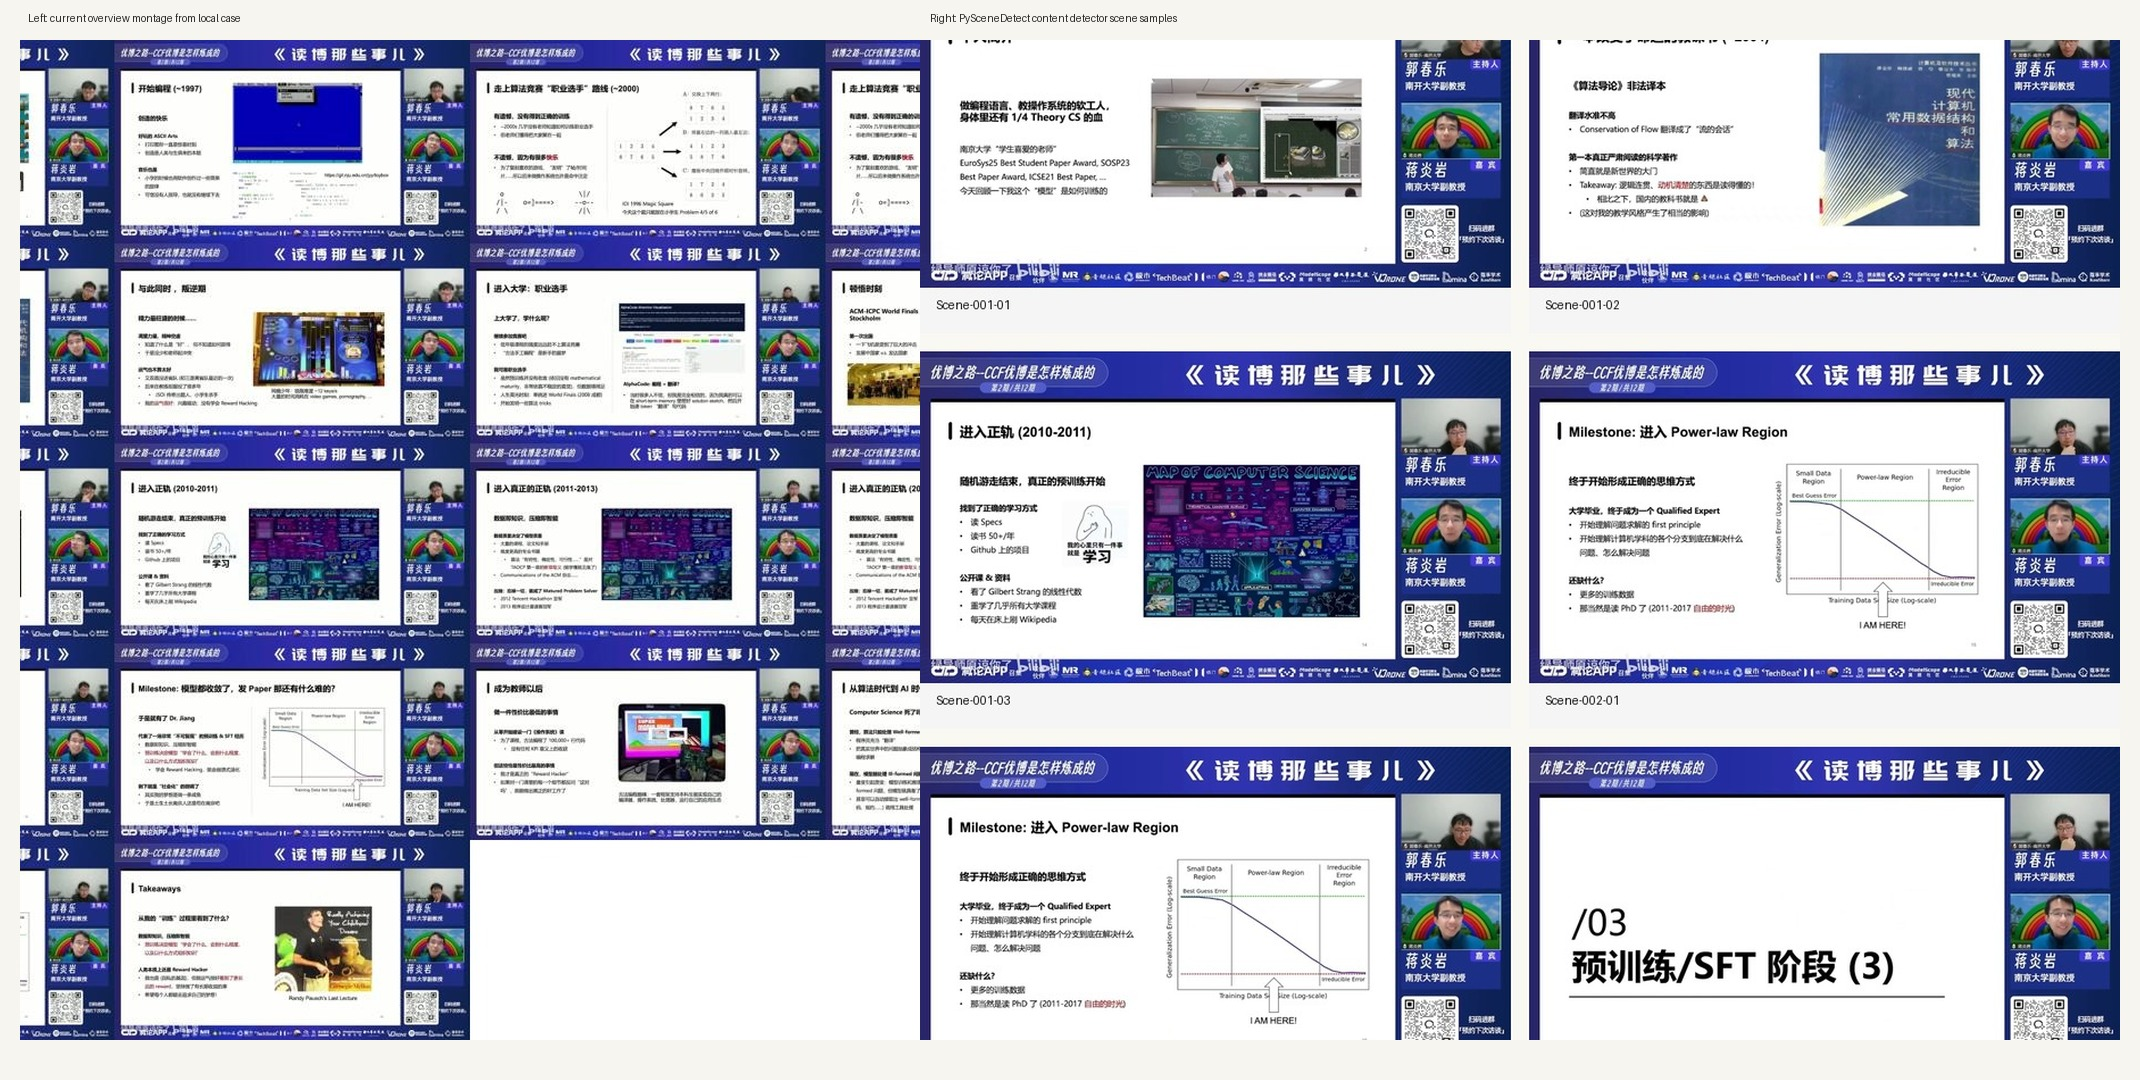
\includegraphics[width=\textwidth]{figures/cover-collage.jpg}
\caption{本地 case 的 overview montage 与 PySceneDetect 内容检测输出样例。来源：左图来自本地 \texttt{overview.jpg}；右图为本轮实验生成的 PySceneDetect scene samples。}
\end{figure}

\subsection{结果：边界检测更适合做候选窗，不适合直接做最终取图}

\begin{table}[H]
\centering
\small
\begin{tabularx}{\textwidth}{p{3.1cm}p{2.2cm}p{2.0cm}Y}
\toprule
方法 & 参数 / 模式 & 检出边界数 & 解释 \\
\midrule
FFmpeg scene score & threshold = 0.10 & 27 & 对亮度 / 内容变化很敏感，易形成较密集候选点 \\
FFmpeg scene score & threshold = 0.15 / 0.20 & 19 & 中等阈值时与 PySceneDetect adaptive 数量接近 \\
FFmpeg scene score & threshold = 0.30 & 6 & 仅保留较大的视觉切换 \\
FFmpeg scene score & threshold = 0.40 & 0 & 默认示例阈值对该 case 过高，直接失效 \\
PySceneDetect \texttt{detect-content} & 默认参数 & 3 & 检出的是较粗的“段落级”视觉变化点 \\
PySceneDetect \texttt{detect-adaptive} & 默认参数 & 18 & 更像稳定版的 dense window proposal \\
\bottomrule
\end{tabularx}
\caption{本地实验中不同方法的边界数量。来源：\texttt{local-experiment-summary.json}。}
\end{table}

\begin{figure}[H]
\centering
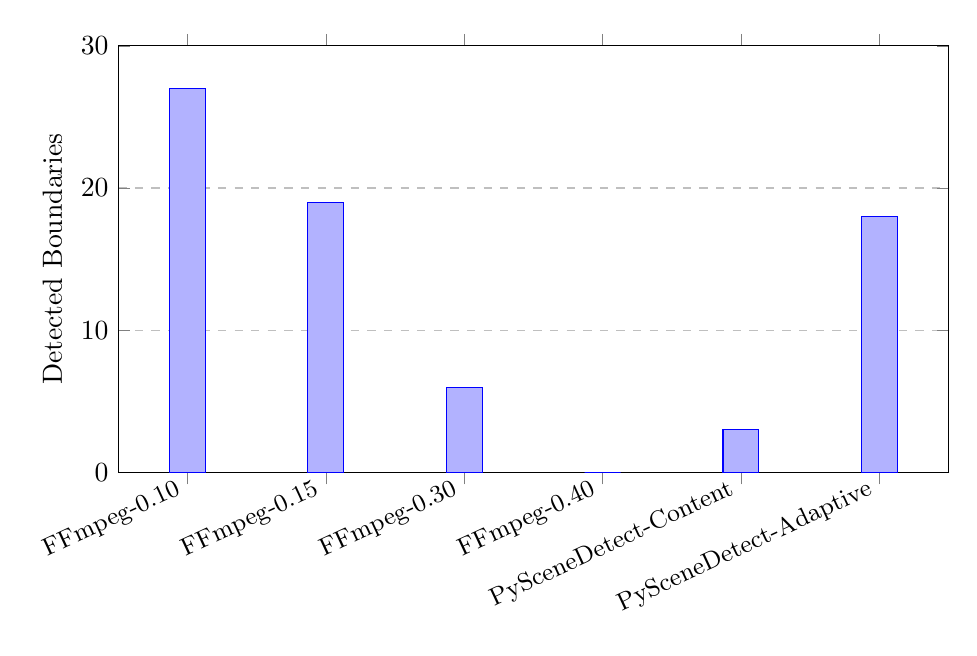
\begin{tikzpicture}
\begin{axis}[
    ybar,
    bar width=13pt,
    width=\textwidth,
    height=7cm,
    ymin=0,
    ymax=30,
    symbolic x coords={FFmpeg-0.10,FFmpeg-0.15,FFmpeg-0.30,FFmpeg-0.40,PySceneDetect-Content,PySceneDetect-Adaptive},
    xtick=data,
    xticklabel style={rotate=25, anchor=east, font=\small},
    ylabel={Detected Boundaries},
    ymajorgrids=true,
    grid style=dashed,
]
\addplot coordinates {
    (FFmpeg-0.10,27)
    (FFmpeg-0.15,19)
    (FFmpeg-0.30,6)
    (FFmpeg-0.40,0)
    (PySceneDetect-Content,3)
    (PySceneDetect-Adaptive,18)
};
\end{axis}
\end{tikzpicture}
\caption{同一视频上，边界检测对参数和算法选择非常敏感。对工程接入来说，最重要的不是“找唯一最优阈值”，而是把它当作一种可配置 probe。}
\end{figure}

\subsection{实验解读}

\begin{itemize}
\item 第一，\textbf{编码兼容性是真实问题}。原始 AV1 视频在默认 PySceneDetect 读帧路径下报错，而 H.264 转码后可以正常运行。这意味着任何准备把 scene detection 做成稳定 runtime 的系统，都要有显式的 \texttt{decode-normalize} 层。
\item 第二，\textbf{PySceneDetect content detector 的 3 个边界更像“粗段落切换”}。它适合作为章节候选或模式切换信号，而不是直接生成最终 figure list。
\item 第三，\textbf{adaptive detector 和 FFmpeg 中等阈值给出了更密的候选点}。这更适合配合 transcript / OCR / layout 去做二次筛选。
\item 第四，\textbf{阈值 0.4 这类官方示例值不应直接照搬}。在你的视频分布里，很多知识视频根本没有那么大的视觉跳变。
\end{itemize}

\begin{findingbox}{与 video-note 直接相关的判断}
如果把 scene detector 放在你现有 pipeline 里，它最合理的位置不是 build 阶段，也不是最终 figure 选择阶段，而是 overview 之后、candidate frame search 之前：先用 cheap detector 生成窗口，再让上层 agent 结合字幕和 case type 决定哪些窗口值得深入。
\end{findingbox}

\section{对你的视频处理方案的落地建议}

\subsection{建议的四层架构}

\begin{figure}[H]
\centering
\resizebox{0.98\textwidth}{!}{%
\begin{tikzpicture}[
    node distance=0.9cm and 0.7cm,
    box/.style={draw, rounded corners, align=center, minimum width=3.1cm, minimum height=1.05cm, fill=blue!4},
    arrow/.style={-Latex, thick}
]
\node[box] (input) {视频输入\\URL / 本地文件};
\node[box, right=of input] (decode) {Decode-Normalize\\编码探测、必要时转码到 H.264};
\node[box, right=of decode] (probe) {Cheap Probe\\overview、FFmpeg scene、PySceneDetect};
\node[box, right=of probe] (route) {Mode Routing\\static-outline / board-heavy / mixed / short-form};

\node[box, below=of decode, minimum width=4.2cm] (candidate) {Candidate Windows\\边界时间点、代表帧、局部时间窗 manifest};
\node[box, right=of candidate, minimum width=4.4cm] (visual) {Visual Understanding\\crop、OCR、layout、slide dedup、可选学习型 SBD};
\node[box, right=of visual, minimum width=4.3cm] (render) {Render Context\\章节、图文预算、provenance、PDF 构建};

\draw[arrow] (input) -- (decode);
\draw[arrow] (decode) -- (probe);
\draw[arrow] (probe) -- (route);
\draw[arrow] (probe) -- (candidate);
\draw[arrow] (route) -- (candidate);
\draw[arrow] (candidate) -- (visual);
\draw[arrow] (visual) -- (render);
\end{tikzpicture}
}
\caption{推荐的结构化中间层。重点不是“先上最强模型”，而是先把可复用 artifact contract 固定下来。}
\end{figure}

\subsection{按阶段推进的技术路线}

\subsubsection{P0：先把最容易稳定的能力做成标准层}

\begin{itemize}
\item 在 overview 之前加入编码探测；对 AV1 / 非主流编码自动做可配置转码。
\item 生成统一的 \texttt{boundary-probe.json} / \texttt{candidate-windows.json}，记录 FFmpeg / PySceneDetect 输出。
\item 不要求 detector 给出最终答案，只要求它给出“哪些时间窗值得进一步看”。
\end{itemize}

\subsubsection{P1：把 PySceneDetect 接成可选增强，而不是默认主线}

\begin{itemize}
\item 对 \texttt{mixed slides/speaker}、\texttt{screen-demo}、\texttt{short-form edited} 视频默认启用；
\item 对 \texttt{static-outline}、\texttt{board-heavy} 只作为辅助，不让其主导 figure selection；
\item 让 transcript window 和 visual boundary 做交集，而不是二选一。
\end{itemize}

\subsubsection{P2：只在确有收益的 case 上评估学习型 SBD}

\begin{itemize}
\item 短视频、高频剪辑、口播和素材混剪混合的视频，才值得重点评估 TransNetV2 / AutoShot。
\item 先做 benchmark 外的小样本 case study，而不是一上来做大规模集成。
\item 如果未来真要接 TransNetV2，优先考虑把模型包装成独立服务或单独环境，避免污染主 runtime。
\end{itemize}

\subsubsection{P3：如果目标升级到章节质量，再看 scene-level / VLM}

\begin{itemize}
\item 当你需要的不只是“图片更准”，而是“章节组织更像人在整理一门课”，scene segmentation 才会变成真正高优先级。
\item 这时应该关注的是 MovieNet / OVSD 这一系工作，以及 Scene-VLM 这样的多模态方法，而不是继续追逐 0.5\% 的 shot F1。
\end{itemize}

\subsection{按视频类型选择技术，而不是按论文热度选择技术}

\begin{table}[H]
\centering
\small
\begin{tabularx}{\textwidth}{p{2.8cm}p{3.0cm}Y}
\toprule
视频类型 & 推荐技术重心 & 原因 \\
\midrule
Static-outline & transcript + 少量 crop + 结构化重绘 & 关键价值在同一页提纲的讲解推进，shot boundary 作用很小 \\
Board-heavy & overview + candidate windows + 最终状态搜索 & 重要的是白板最终可读状态，不是每次小变化都切一刀 \\
Low-visual commentary & transcript / semantic organization 为主 & 大量边界检测只会制造无意义截图 \\
Mixed slides / speaker & PySceneDetect + transcript 对齐 + crop / OCR & 视觉段落切换较明显，detector 能显著缩小候选空间 \\
Short-form edited video & 学习型 SBD 值得重点评估 & 高频转场、复杂编辑更能体现 TransNetV2 / AutoShot 价值 \\
\bottomrule
\end{tabularx}
\caption{对你当前场景最重要的不是“哪个模型最强”，而是“哪个模型在哪类视频上值得启动”。}
\end{table}

\section{结论与后续问题}

\subsection{已经有强证据支持的判断}

\begin{itemize}
\item Shot boundary detection 是重要中间能力，但不足以单独解决 video-note。
\item 公开可复现的 shot-level 主线在近几年没有爆炸式新进展，公开社区里最值得参考的代表仍是 TransNetV2 与 AutoShot。
\item 截至 2026-03-26，2025+ 的新强模型主要分布在两条线：scene segmentation 的 MASRC / Scene-VLM，以及 GEBD 的 Structured Context Learning / ESTimator / DiffGEBD。
\item PySceneDetect 和 FFmpeg 对你现在的工程 ROI 很高，足以作为第一阶段接入。
\item 真实 pipeline 必须考虑视频编码兼容性，本轮本地实验里的 AV1 失败就是直接证据。
\item 如果长期目标是章节组织和更像人类整理的文档结构，scene-level、多模态、可解释方法更值得中长期关注。
\end{itemize}

\subsection{较大概率成立但仍需你们自己验证的判断}

\begin{itemize}
\item 对 `mixed slides/speaker` 和 `screen-demo`，PySceneDetect 很可能已经能带来明显收益。
\item 对 `static-outline` 和 `board-heavy`，学习型 SBD 很可能收益有限，甚至会带来过多重复候选图。
\item 对短视频和高频剪辑场景，如果你们之后想做 clip chaptering 或 auto-highlights，AutoShot 系统值得专门评估。
\end{itemize}

\subsection{目前仍未知的关键问题}

\begin{itemize}
\item 你们自己的视频分布里，到底哪一类 case 占主流，是否真的值得为少量高编辑密度视频维护重模型。
\item 章节质量的主要瓶颈究竟在视觉切分、还是在 transcript semantics、还是在 PDF 渲染中间层。
\item Scene-level / VLM 方法在你们的中文讲解视频、板书视频和 screen-demo 视频上，是否真的比 rule-based 中间层更有性价比。
\end{itemize}

\appendix

\section{来源清单}

\small
\begin{longtable}{p{1.7cm}p{1.8cm}p{4.0cm}p{6.0cm}}
\toprule
Source ID & 模态 & 标题 / 标签 & 链接或路径 \\
\midrule
\endfirsthead
\toprule
Source ID & 模态 & 标题 / 标签 & 链接或路径 \\
\midrule
\endhead
L1 & Local report & 既有背景报告 & \path{/home/fanghaotian/Desktop/src/agent-basic-skill/reports/2026-03-26-video-note-visualize-deepresearch/report.tex} \\
L2 & Local runtime & video-note-pipeline README & \path{/home/fanghaotian/Desktop/src/video-note-pipeline/README.md} \\
L3 & Local case & BV1cptBzFE5Q retrospective & \path{/home/fanghaotian/Desktop/src/video_notes/evlove/WORKFLOW_RETROSPECTIVE_BV1cptBzFE5Q_2026-03-25.md} \\
L4 & Local case & BV1GZw9zcEdJ retrospective & \path{/home/fanghaotian/Desktop/src/video_notes/evlove/WORKFLOW_RETROSPECTIVE_BV1GZw9zcEdJ_2026-03-25.md} \\
L5 & Local case & BV1oTwkzvEFu case directory & \path{/home/fanghaotian/Desktop/src/video_notes/20260326-023015-8718c4102fe9dirty-BV1oTwkzvEFu} \\
L6 & Local experiment & 本轮实验摘要 JSON & \path{/home/fanghaotian/Desktop/src/agent-basic-skill/reports/2026-03-26-shot-boundary-scene-detection-deepresearch/artifacts/local-experiment-summary.json} \\
W1 & Web official & TransNetV2 README & \url{https://github.com/soCzech/TransNetV2/blob/master/README.md} \\
W2 & Paper & TransNetV2 paper & \url{https://arxiv.org/abs/2008.04838} \\
W3 & Web official & PySceneDetect CLI docs & \url{https://www.scenedetect.com/docs/latest/cli.html} \\
W4 & Web official & FFmpeg filters docs & \url{https://ffmpeg.org/ffmpeg-filters.html} \\
W5 & Web official & AutoShot README & \url{https://github.com/wentaozhu/AutoShot} \\
W6 & Paper & AutoShot paper & \url{https://arxiv.org/abs/2304.06116} \\
W7 & Web official & ClipShots README & \url{https://github.com/Tangshitao/ClipShots} \\
W8 & Paper & ClipShots paper & \url{https://arxiv.org/abs/1808.04234} \\
W9 & Paper & MovieNet / MovieScenes paper & \url{https://arxiv.org/abs/2004.02678} \\
W10 & Paper & Neighbor Relations Matter in Video Scene Detection & \url{https://openaccess.thecvf.com/content/CVPR2024/html/Tan_Neighbor_Relations_Matter_in_Video_Scene_Detection_CVPR_2024_paper.html} \\
W11 & Paper & Scene-VLM paper & \url{https://arxiv.org/abs/2512.21778} \\
W12 & Web official & BBC / RAI dataset portal & \url{https://aimagelab.ing.unimore.it/imagelab/researchActivity.asp?idActivity=19} \\
W13 & Derived search & arXiv recent shot-boundary search & \path{/home/fanghaotian/Desktop/src/agent-basic-skill/reports/2026-03-26-shot-boundary-scene-detection-deepresearch/artifacts/arxiv-shot-boundary-recent.json} \\
W14 & Paper & MASRC / Modality-Aware Shot Relating and Comparing for Video Scene Detection & \url{https://arxiv.org/abs/2412.17238} \\
W15 & Web official & MASRC GitHub repo & \url{https://github.com/ExMorgan-Alter/MASRC} \\
W16 & Paper & Structured Context Learning for Generic Event Boundary Detection & \url{https://arxiv.org/abs/2512.00475} \\
W17 & Paper & Online Generic Event Boundary Detection & \url{https://arxiv.org/abs/2510.06855} \\
W18 & Paper & DiffGEBD / Generic Event Boundary Detection via Denoising Diffusion & \url{https://arxiv.org/abs/2508.12084} \\
W19 & Web official & DiffGEBD GitHub repo & \url{https://github.com/JaejunHwang/DiffGEBD} \\
\bottomrule
\end{longtable}

\section{本地实验关键时间点}

\begin{itemize}
\item PySceneDetect \texttt{detect-content} 检出的 3 个主要边界为：00:14:02.667、00:15:12.600、00:17:27.267。
\item PySceneDetect \texttt{detect-adaptive} 共检出 18 个边界，更适合作为候选窗口而非直接章节。
\item FFmpeg scene threshold 从 0.10 到 0.40 的结果分别为 27、19、6、0 个边界，显示参数敏感性显著。
\end{itemize}

\end{document}
